\documentclass[10pt,french]{article}

\input preambule_2013
\RegleEntete


\newcommand\competences{
\setcounter{exo}{0}\renewcommand\arraystretch{1.2}
\begin{tabular}{ll} Nom : \\[5pt] Prénom : \end{tabular}
\hfill
\textbf{Note :}
\begin{tabular}{|c|}
\hline
\slashbox{\Huge\bfseries\phantom{10}}{\Huge\bfseries 10}\\
\hline
\end{tabular}\renewcommand\arraystretch{1}
\[***\]
}

\entete{\premiere \stmg}{Statistiques \\ Indicateurs de position}{A}
\pieddepage{}{}{}


\begin{document}
\competences

On relève la pointure de $25$ personnes. Les données sont recueillies dans le tableau ci-dessous :

\begin{center}
\renewcommand\arraystretch{1.5}
    \begin{tabular}{|>\bfseries M{2cm}|*{7}{M{1.2cm}|}c|}
        \hline
            Pointures & 36 & 37 & 38 & 39 & 40 & 41 & 42 & Total \\
        \hline
            Effectifs & 1 & 2 & 1 & 3 & 5 & 10 & 3 & \\
        \hline
            Fréquence (en \%) & & & & & & & & \\
        \hline
            {\footnotesize Fréq. Cumulée Croissante\par (en \%)} & & & & & & & & \\
        \hline
    \end{tabular}
\renewcommand\arraystretch{1.5}
\end{center}

\begin{enumerate}
    \item Compléter le tableau avec des valeurs exactes.
    \item En détaillant précisément les étapes, déterminer la valeur exacte de la moyenne $\overline m$ de cette série statistique.
    \item En détaillant précisément la démarche, déterminer :
        \begin{itemize}
            \item la médiane $M_e$ et interpréter le résultat ;
            \item le premier quartile $Q_1$ et interpréter le résultat ;
            \item le troisième quartile $Q_3$ et interpréter le résultat.
        \end{itemize}
    \item Sur le repère de gauche ci-dessous, dessiner le diagramme en bâton correspondant à cette série statistique.
    \item Sur le repère de droite ci-dessous, dessiner le polygone des fréquences cumulées croissantes correspondant à cette série statistique.
    \item Utiliser le graphique précédent pour \textbf{lire} une valeur de la médiane, du premier et du troisième quartile. Faire apparaître les pointillés sur le graphique.
    \item Quel pourcentage de personnes ont une pointure \textbf{strictement supérieure} à $37$ ?
\end{enumerate}
\medskip

\begin{center}
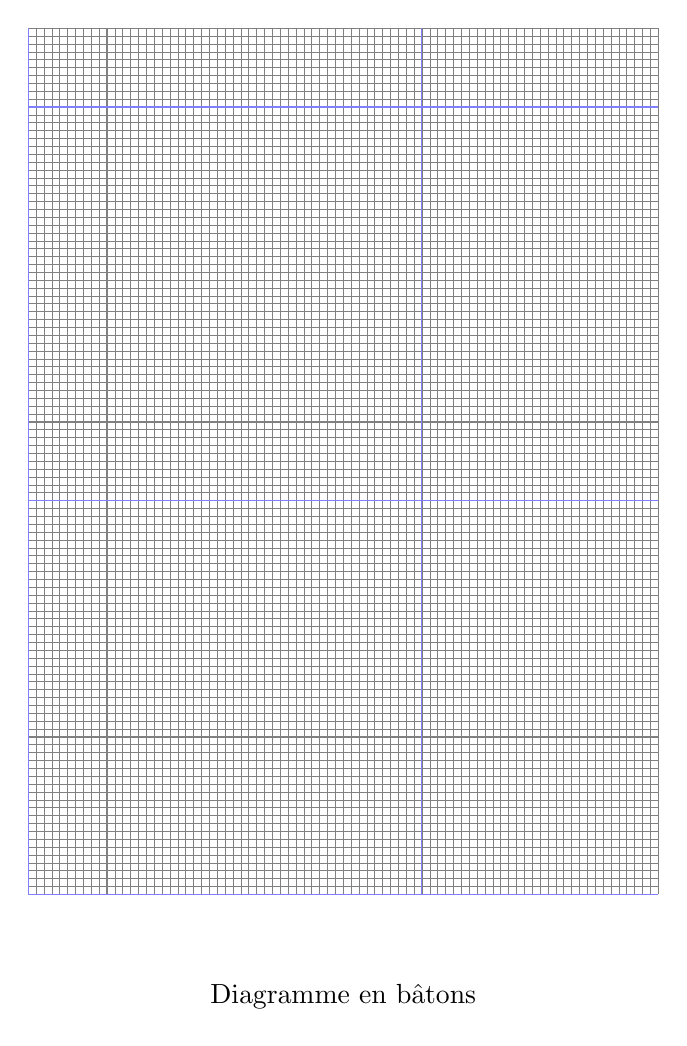
\begin{tikzpicture}
	% Dimensions du repere
	\def\xmin{0} \def\xmax{8} \def\ymin{0} \def\ymax{11}
	% Grilles
	\draw [step=0.1,gray,very thin]  (\xmin,\ymin) grid (\xmax,\ymax);
	\draw [step=1,gray,thin] (\xmin,\ymin) grid (\xmax,\ymax);
	\draw [step=5,thin,color=blue!50]  (\xmin,\ymin) grid (\xmax,\ymax);
	% Clip pour que les figures ne sortent pas du cadre
%	\clip (\xmin,\ymin) rectangle (\xmax,\ymax);
    \draw (4,-1.3) node {Diagramme en bâtons};
\end{tikzpicture}
\hfill
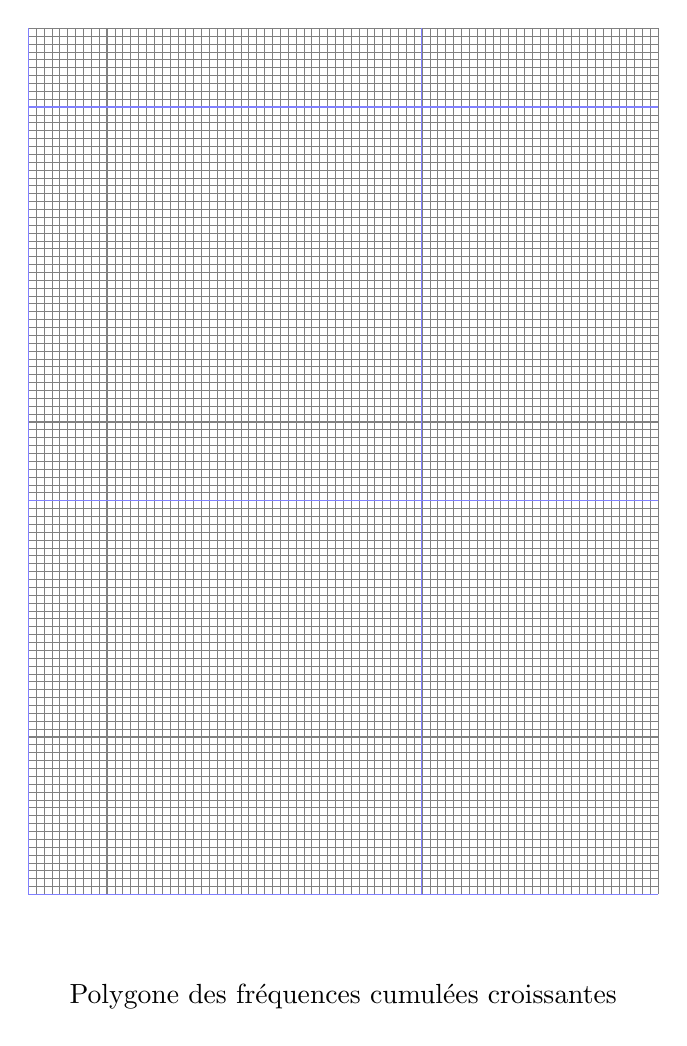
\begin{tikzpicture}
	% Dimensions du repere
	\def\xmin{0} \def\xmax{8} \def\ymin{0} \def\ymax{11}
	% Grilles
	\draw [step=0.1,gray,very thin]  (\xmin,\ymin) grid (\xmax,\ymax);
	\draw [step=1,gray,thin] (\xmin,\ymin) grid (\xmax,\ymax);
	\draw [step=5,thin,color=blue!50]  (\xmin,\ymin) grid (\xmax,\ymax);
	% Clip pour que les figures ne sortent pas du cadre
%	\clip (\xmin,\ymin) rectangle (\xmax,\ymax);
    \draw (4,-1.3) node {Polygone des fréquences cumulées croissantes};
\end{tikzpicture}
\end{center}

\clearpage

%--------------------------------------------------------------------------------------------------------------------------------------------------------------------------
%                           SUJET B
%--------------------------------------------------------------------------------------------------------------------------------------------------------------------------

\entete{\premiere \stmg}{Statistiques \\ Indicateurs de position}{B}
\competences

On relève la pointure de $25$ personnes. Les données sont recueillies dans le tableau ci-dessous :

\begin{center}
\renewcommand\arraystretch{1.5}
    \begin{tabular}{|>\bfseries M{2cm}|*{7}{M{1.2cm}|}c|}
        \hline
            Pointures & 39 & 40 & 41 & 42 & 43 & 44 & 45 & Total \\
        \hline
            Effectifs & 5 & 8 & 4 & 3 & 1 & 1 & 3 & \\
        \hline
            Fréquence (en \%) & & & & & & & & \\
        \hline
            {\footnotesize Fréq. Cumulée Croissante\par (en \%)} & & & & & & & & \\
        \hline
    \end{tabular}
\renewcommand\arraystretch{1.5}
\end{center}

\begin{enumerate}
    \item Compléter le tableau avec des valeurs exactes.
    \item En détaillant précisément les étapes, déterminer la valeur exacte de la moyenne $\overline m$ de cette série statistique.
    \item En détaillant précisément la démarche, déterminer :
        \begin{itemize}
            \item la médiane $M_e$ et interpréter le résultat ;
            \item le premier quartile $Q_1$ et interpréter le résultat ;
            \item le troisième quartile $Q_3$ et interpréter le résultat.
        \end{itemize}
    \item Sur le repère de gauche ci-dessous, dessiner le diagramme en bâton correspondant à cette série statistique.
    \item Sur le repère de droite ci-dessous, dessiner le polygone des fréquences cumulées croissantes correspondant à cette série statistique.
    \item Utiliser le graphique précédent pour \textbf{lire} une valeur de la médiane, du premier et du troisième quartile. Faire apparaître les pointillés sur le graphique.
    \item Quel pourcentage de personnes ont une pointure \textbf{strictement supérieure} à $40$ ?
\end{enumerate}
\medskip

\begin{center}
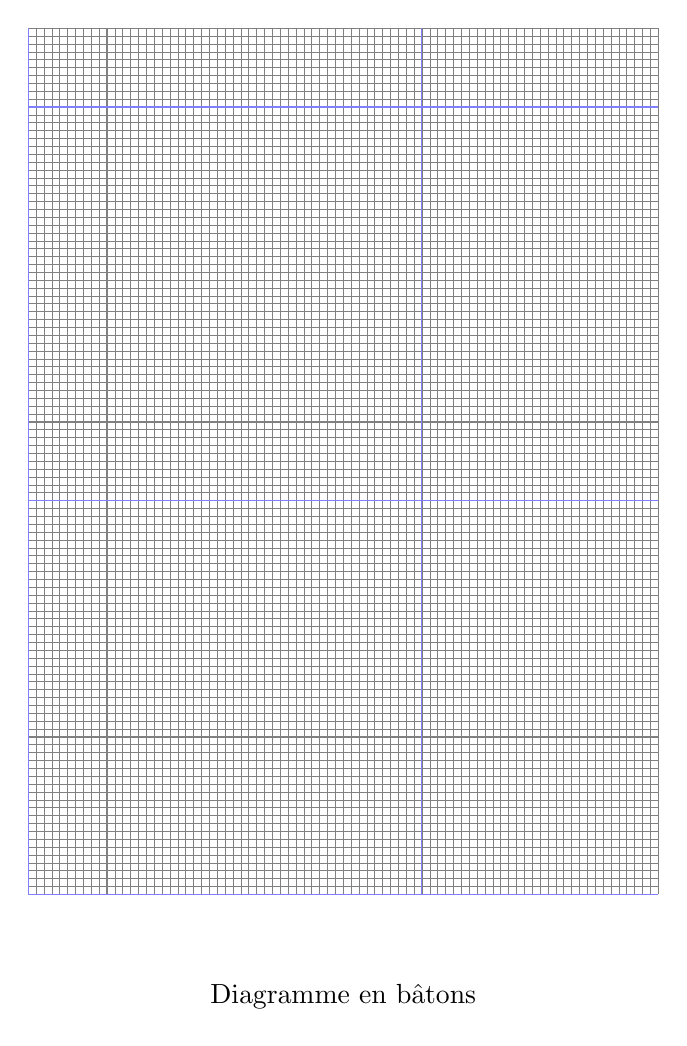
\begin{tikzpicture}
	% Dimensions du repere
	\def\xmin{0} \def\xmax{8} \def\ymin{0} \def\ymax{11}
	% Grilles
	\draw [step=0.1,gray,very thin]  (\xmin,\ymin) grid (\xmax,\ymax);
	\draw [step=1,gray,thin] (\xmin,\ymin) grid (\xmax,\ymax);
	\draw [step=5,thin,color=blue!50]  (\xmin,\ymin) grid (\xmax,\ymax);
	% Clip pour que les figures ne sortent pas du cadre
%	\clip (\xmin,\ymin) rectangle (\xmax,\ymax);
    \draw (4,-1.3) node {Diagramme en bâtons};
\end{tikzpicture}
\hfill
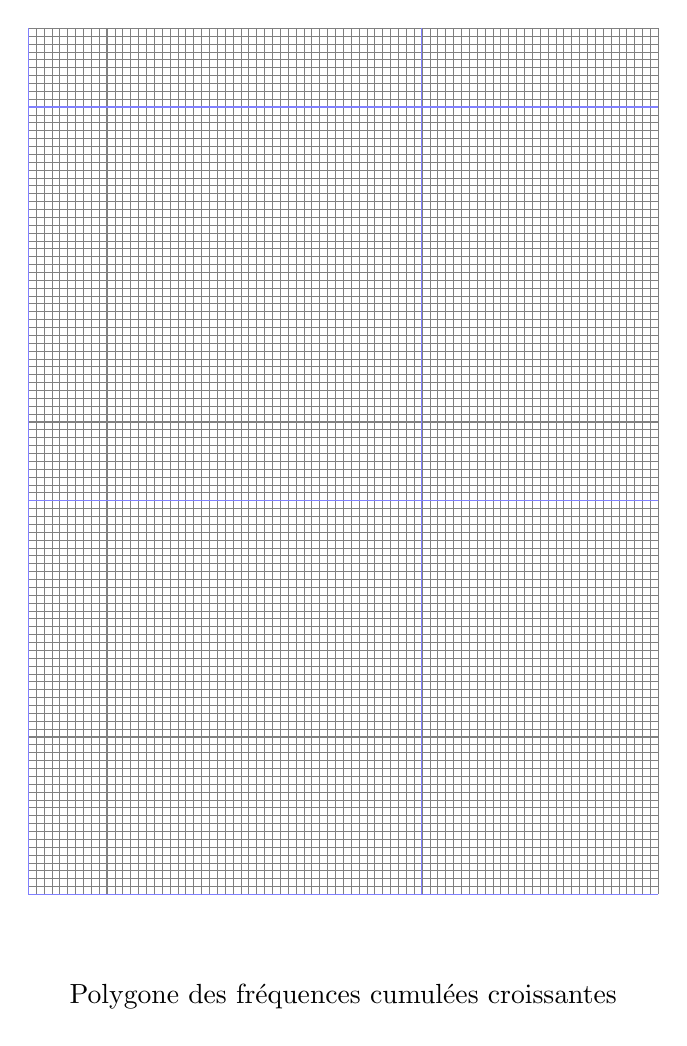
\begin{tikzpicture}
	% Dimensions du repere
	\def\xmin{0} \def\xmax{8} \def\ymin{0} \def\ymax{11}
	% Grilles
	\draw [step=0.1,gray,very thin]  (\xmin,\ymin) grid (\xmax,\ymax);
	\draw [step=1,gray,thin] (\xmin,\ymin) grid (\xmax,\ymax);
	\draw [step=5,thin,color=blue!50]  (\xmin,\ymin) grid (\xmax,\ymax);
	% Clip pour que les figures ne sortent pas du cadre
%	\clip (\xmin,\ymin) rectangle (\xmax,\ymax);
    \draw (4,-1.3) node {Polygone des fréquences cumulées croissantes};
\end{tikzpicture}
\end{center}


\end{document} 